%!TEX encoding = UTF-8 

\chapter{Robot Platform and Software Setup}
\label{chap:robot_platform}

\begin{figure}
\centering
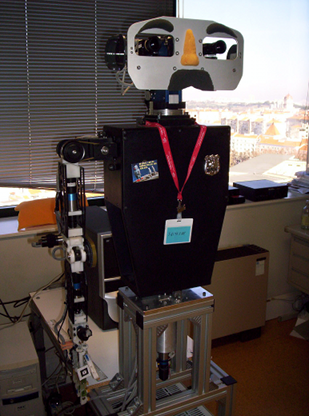
\includegraphics{figures/balta_relaxed}
\caption[Baltazar humanoid robot in relax position]{Baltazar humanoid robot in relax position.}
\label{img:balta_relaxed}
\end{figure}

In 2004, Computer and Robot Vision Laboratory~\cite{link:vislab} at IST in Lisbon developed a humanoid robot platform, ``Baltazar''~\cite{lopes:2004}\index{Baltazar}, which was used for this work. Baltazar, shown in Fig.~\ref{img:balta_relaxed}, is an anthropomorphic torso that features a binocular head as well as an arm and a hand. It was built as a system that mimics human arm-hand kinematics as closely as possible, despite the relatively simple design.

Baltazar is well suited (and was designed) for research in imitation\index{imitation}, skill transfer and visuomotor coordination. The design of Baltazar was driven by these constraints:
\begin{itemize}
\item the robot should resemble a human torso;

\item the robot kinematics should be able to perform human-like movements and gestures, as well as to allow a natural interaction with objects during grasping;

\item payload should be at least 500 g (including the hand);

\item force detection should be possible;

\item the robot should be easy to maintain and be low cost (it contains regular DC motors with reduced backlash and off-the-shelf mechanical parts).
\end{itemize}

In this section we will summarize mechanical and kinematic details of Baltazar, its sensors and technology. More details (such as the design of the 11-\ac{DOF} hand of Baltazar, not actually used in this thesis work as we focus on grasping \emph{preparation}) can be found in~\cite[p.~113]{lopes:phd}.

A software library used to develop programs for Baltazar, called \ac{YARP}, is used extensively in the whole \ac{RobotCub} developers community and in the implementation of this thesis, therefore \ac{YARP} and its middleware mechanisms will also be described; other secondary software tools that we used will be cited.

%%%%%%%%%%%%%%%%%%%%%%
%%%%%%%%%%%%%%%%%%%%%%
\section{Kinematic Description of Baltazar}

Robot kinematics studies the \emph{motion} of robots, thus taking into account the positions, velocities and accelerations of robot links, but without regard to the forces that actually cause the motion (whose study belongs to robot dynamics): robot kinematics uses just geometrical constraints. The kinematics of manipulators involves the study of the geometric- and time-based properties of motion, in particular how the various links move with respect to one another and with time.

The vast majority of robots belong to the \emph{serial} link manipulator class, which means that it comprises a set of bodies called \emph{links} in a chain, connected by \emph{joints}\footnote{To be more accurate, parallel link and serial/parallel hybrid structures are theoretically possible, although they are not common.}. Each joint has one \ac{DOF}, either translational or rotational; for example, the anthropomorphic arm used for the work of this thesis has 6 rotational \acp{DOF}.

For a manipulator with $n$ joints numbered from $1$ to $n$, there are $n+1$ links, numbered from $0$ to $n$. Link $0$ is the base of the manipulator, while link $n$ carries the end-effector. Joint $i$ connects links $i$ and $i-1$.

% ?
The kinematic model of a robot expresses how its several components move among themselves, achieving a transformation between different configuration spaces. The ``spaces'' mentioned here are the ones of the Cartesian geometric world workspace, as opposed to less-intuitive spaces that are directly associated with the robot's joint parameters, which are usually~\cite{craig, sciavicco_siciliano} denoted as a vector $\mathbf{q}$.

The following types of kinematics approaches are commonly studied in robotics:
\begin{description}
\item[forward kinematics] computes the position of a point in space (typically, that of the end-effector), given the values of the joint parameters (lengths and angles);

\item[inverse kinematics] computes all the joint parameters, given a point in space that the end-effector must lie on;

\item[forward velocity kinematics] (or forward differential kinematics) computes the velocity of a point in space, given the derivatives of the joint parameters;

\item[inverse velocity kinematics] (or inverse differential kinematics) computes the derivatives, i.e., velocities of joint parameters, given spatial velocities.
\end{description}

Forward kinematics (also known as direct kinematics) is the problem of transforming the joint positions of a robot to its end-effector pose. In other words, it is the computation of the position and orientation of a robot's end-effector as a function of its joint angles. For example, given a serial chain of $n$ links and letting $\theta_i$ be the angle of link $i$, then the reference frame of link $n$ relative to link $0$ is
\[
\leftidx{^0} {\mathbf{T}}_n = \prod_{i=1}^n  \leftidx{^{i-1}}{\mathbf{T}}_i (\theta_i)
\]
where $\leftidx{^{i-1}}{\mathbf{T}}_i(\theta_i)$ is the transformation matrix from the frame of link $i$ to that of link $i-1$.


%%%%%%%%%%%%%%%
\subsection{Kinematic Notation}
\index{Denavit-Hartenberg (DH)}
\index{Denavit-Hartenberg (DH)!SDH} \index{Denavit-Hartenberg (DH)!MDH}

\begin{figure}
\centering
\subfloat[][\acl{SDH} (\acs{SDH}) convention.]
{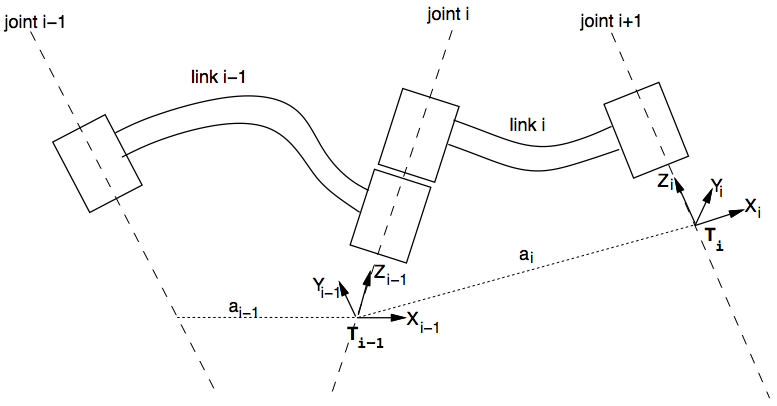
\includegraphics[width=.45\columnwidth]{figures/standard_dh} } \quad
% %necessary to prevent line break
\subfloat[][\acl{MDH} (\acs{MDH}) convention.]
{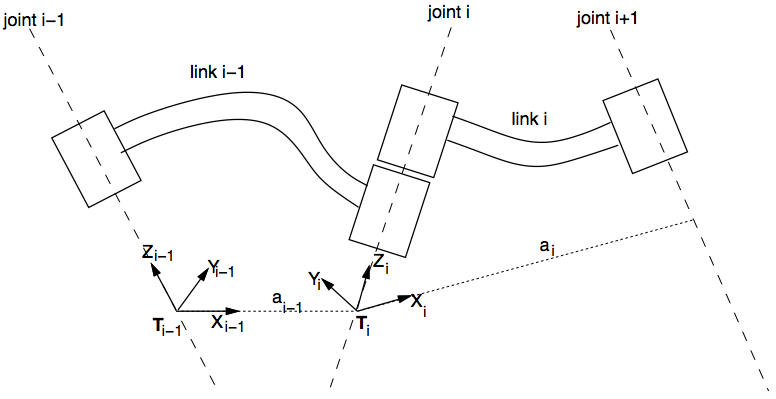
\includegraphics[width=.45\columnwidth]{figures/modified_dh} }

\caption[Different forms of \acs{DH} notation]{Different forms of \ac{DH} notation. Note: $a_i$ always indicates the length of link $i$, but the displacement it represents is between the origins of frame $i$ and frame $i+1$ in the standard form, between frames $i-1$ and $i$ in the modified form.

%Picture: Robotics Toolbox for MATLAB.
}
\label{fig:dh}
\end{figure}

A word of advice on the study and notation of kinematics: in robotics literature, at least two related but different conventions to model serial manipulator kinematics go by the name \ac{DH}, however they actually vary in a few details related to the assignment of reference frames to the rigid bodies (links) of robots.

These differences among \ac{DH} parameterizations are rarely acknowledged (with the exception of~\cite{corke:1996}). Typically, an author chooses one of the existing \ac{DH} notations, writes down ``this is the Denavit-Hartenberg convention'' then sticks to it from that moment on. One should, however, pay attention to which \ac{DH} formulation is being used and understand it.

Two different methodologies, shown in Fig.~\ref{fig:dh}, have been established to assign coordinate frames:
\begin{enumerate}
\item \ac{SDH} form, also known as ``unmodified'' \ac{DH} convention: frame $i$ has its origin along the axis of joint $i+1$.

\item \ac{MDH} form: frame $i$ has its origin along the axis of joint $i$.
\end{enumerate}

\ac{MDH} is commonly used in the literature on manipulator mechanics, and the (forward and inverse) kinematics approaches for Baltazar that exist so far, have in fact followed the \ac{MDH} form. However, further on we will see cases where it is practical to make a change of representation to \ac{SDH} to model the arm of Baltazar by the means of publicly-available robotics simulation tools.

The difference between \ac{SDH} and \ac{MDH} is the following\marginpar{Difference between \ac{SDH} and \ac{MDH}.}. In \ac{SDH}, we position the origin of frame $i$ along the axis of joint $i+1$. With \ac{MDH}, instead, frame $i$ has its origin along the axis of joint $i$.

A point to stress is that the choices of the various reference frames to assign (with \acs{SDH} or with \acs{MDH}) are \emph{not unique}, even under the constraints that need to be enforced among consecutive links. For example, the origin of the first reference frame $O_0$ can be arbitrarily positioned anywhere on the first joint axis. Thus, it is possible to derive different, equally valid, coordinate frame assignments for the links of a given robot. On the other hand, the final matrix that transforms from the base to the end effector, $\leftidx{^n}{\mathbf{T}}_0$, must be the same---regardless of the intermediate frame assignments.

For a detailed description of \ac{DH} conventions and the meaning of the four parameters ($a$: link length; $\alpha$: link twist; $d$: link offset; $\theta$: joint angle) refer, for example, to:
\begin{itemize}
\item \cite{spong}, which explains \ac{SDH} thoroughly; Chapter~3 is publicly available\footnote{\url{http://www.cs.duke.edu/brd/Teaching/Bio/asmb/current/Papers/chap3-forward-kinematics.pdf}};

\item \cite{craig} for \ac{MDH}; or

\item \cite{corke:1996} (both parameterizations).
\end{itemize}



%\subsubsection{\ac{SDH} link transform}

If we use the \ac{SDH} representation, the following $4 \times 4$ homogeneous transformation matrix
%
\begin{equation}
\label{eq:sdh_transf}
\leftidx{^{i-1}}{\mathbf{A}}_i = 
\begin{bmatrix}
\cos\theta_i & -\sin\theta_i \cos\alpha_i & \sin\theta_i \sin\alpha_i & a_i \cos\theta_i \\
\sin\theta_i & \cos\theta_i \cos\alpha_i & -\cos\theta_i \sin\alpha_i & a_i \sin\theta_i \\
0 & \sin\alpha_i & \cos\alpha_i & d_i \\
0 & 0 & 0 & 1
\end{bmatrix}
\end{equation}
%
represents each link's coordinate frame with respect to the previous link's coordinate system, i.e.,
\begin{equation}\label{eq:transf}
\leftidx{^0}{\mathbf{T}}_i = \leftidx{^0}{\mathbf{T}}_{i-1} \quad \leftidx{^{i-1}}{\mathbf{A}}_i
\end{equation}
where $\leftidx{^0}{\mathbf{T}}_i$ is the homogeneous transformation describing the pose (position and orientation) of coordinate frame $i$ with respect to the world coordinate system $0$.

%\subsubsection{\ac{MDH} link transform}

With \ac{MDH}, Eq.~\ref{eq:transf} still holds, however the homogeneous transformation matrix assumes the following form (instead of Eq.~\ref{eq:sdh_transf}):
%
\begin{equation}\label{eq:mdh_transf}
\leftidx{^{i-1}}{\mathbf{A}}_i = 
\begin{bmatrix}
\cos\theta_i & -\sin\theta_i & 0 & a_{i-1} \\
\sin\theta_i \cos\alpha_{i-1} & \cos\theta_i \cos\alpha_{i-1} & -\sin\alpha_{i-1} & d_i \sin\alpha_{i-1} \\
\sin\theta_i \sin\alpha_{i-1} & \cos\theta_i \sin\alpha_{i-1} & \cos\alpha_{i-1} & d_i \cos\alpha_{i-1} \\
0 & 0 & 0 & 1
\end{bmatrix}
\end{equation}




%%%%%%%%%%%%%%%
\subsection{Head Structure}
\label{sec:balta_head} \index{Baltazar!head}

\begin{figure}
\centering
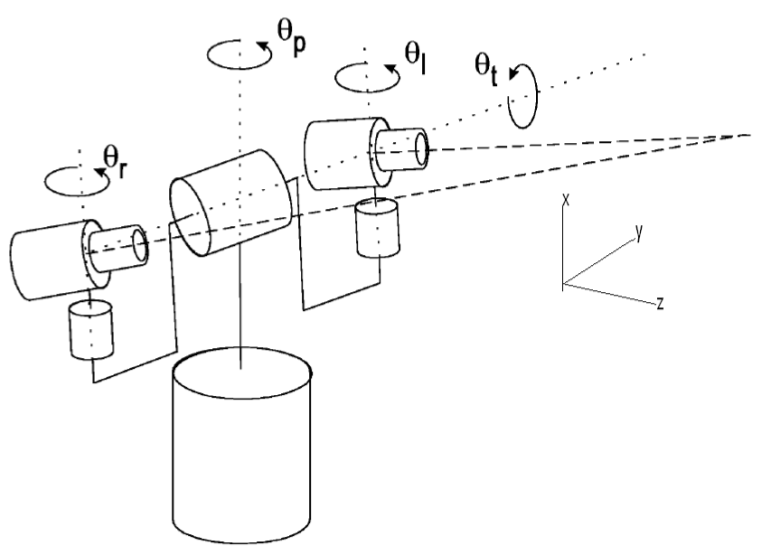
\includegraphics[scale=0.4]{figures/balta_head_scheme}
\caption[Scheme of Baltazar robotic head]{Scheme of Baltazar robotic head, code-named ``Medusa''~\cite{bernardino:1999}. The meaning of the four joint angles $\theta_l, \theta_r, \theta_p$ and $\theta_t$ is explained in Table~\ref{tab:balta_head_joints}.}
\label{img:balta_head_scheme}
\end{figure}

\begin{table}
\caption[Joint angles of Baltazar robotic head]{Joint angles of Baltazar robotic head.}
\label{tab:balta_head_joints}
\centering
\medskip
\begin{tabular}{*{2}{l}} % table with 2 left-aligned columns
\toprule
angle & description \\
\otoprule
$\theta_l$ & left eye camera vergence \\
\midrule
$\theta_r$ & right eye camera vergence \\
\midrule
$\theta_p$ & pan (neck rotation) \\
\midrule
$\theta_t$ & tilt (head rotation) \\
\bottomrule
\end{tabular}
\end{table}

The mechanical and geometrical structure of the robotic head used for this thesis work can be seen in Fig.~\ref{img:balta_head_scheme}, which shows the four \acp{DOF} of the head, all of which are rotational: neck rotation (pan), head elevation (tilt), left eye vergence, and right eye vergence.

\begin{figure}
\centering
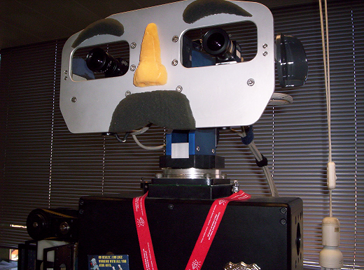
\includegraphics{figures/balta_head_real}
\caption[Real Baltazar robotic head]{Real Baltazar robotic head.}
\label{img:balta_head_real}
\end{figure}

A view of the real Baltazar robotic head, along with its two cameras, can be seen in Fig.~\ref{img:balta_head_real}.

Manual adjustments can be made to align the vergence and elevation axes of rotation with the optical centres of the cameras. Inter-ocular distance (baseline) can also be modified. \ac{MDH} parameters of the head are displayed in Table~\ref{tab:balta_head_mdh}.

\begin{table}
\caption[\acs{MDH} parameters of Baltazar binocular head]{A possible \ac{MDH} parameterization of the left eye of the binocular head of Baltazar, taken from~\cite{lopes:2004}. $B$ is the baseline distance between the two eyes.}
\label{tab:balta_head_mdh}
\centering
\medskip
\begin{tabular}{*{5}{l}} % table with 5 left-aligned columns
\toprule
Joint $i$ & $a_{i-1}$ [cm] & $d_i$ [cm]& $\alpha_{i-1}$ [$\degree$] & $\theta_i$ [$\degree$] \\
\otoprule
$1$ & $0$ & $0$ & $0$ & $\theta_p$ \\
\midrule
$2$ & $15$ & $0$ & $-\pi$ & $\theta_t$ \\
\midrule
$3$ & $0$ & $B/2$ & $\pi$ & $0$ \\
\midrule
$4$ & $0$ & $0$ & $\pi$ & $\theta_r$ \\
\bottomrule
\end{tabular}
\end{table}

Let $\leftidx{^2}{\mathbf{P}}$ denote the 3D coordinates of point $\mathbf{P}$ expressed in eye coordinates. If we denote by $\leftidx{^A}{\mathbf{P}}$ the coordinates of $\mathbf{P}$ expressed in the arm base (shoulder) coordinate system, this relation holds:
%
% I removed the _h subscript in the two last T's
\begin{equation}
\leftidx{^A}{\mathbf{P}} = \leftidx{^A}{\mathbf{T}}_H \quad \leftidx{^1}{\mathbf{T}}_0 \quad \leftidx{^1}{\mathbf{T}}_2 \quad \leftidx{^2}{\mathbf{P}}
\end{equation}
%
where the head--arm transformation $\leftidx{^A}{\mathbf{T}}_H$ is given by
%
\begin{equation}\label{eq:head_to_arm}
\leftidx{^A}{\mathbf{T}}_H =	\begin{bmatrix}
						0 & 0 & 1 & -27 \\
						-1 & 0 & 0 & 0 \\
						0 & -1 & 0 & 29.6 \\
						0 & 0 & 0 & 1
						\end{bmatrix}
\end{equation}
and the translation values of the first three rows of the last column of Eq.~\ref{eq:head_to_arm} are expressed in centimetres.

%%%%%%%%%%%%%%%%%%%%%%%%%%%
\subsection{Baltazar and Its Anthropomorphic Arm}
\index{Baltazar!anthropomorphic arm}

Baltazar has an anthropomorphic arm inspired from human arms. However, given the complexity of articulations that a human arm can present, it is still not viable to reproduce one from a technology standpoint. Thus, some simplifications are due, and unfortunately they bring along a loss of maneuverability. The anthropomorphic arm of Baltazar is a fair compromise between complexity and imitation of a human arm.

\begin{figure}
\centering
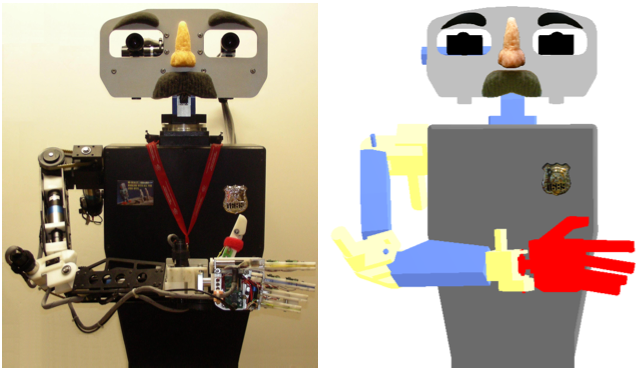
\includegraphics[scale=0.5]{figures/balta_real_cad}
\caption[Real Baltazar and its CAD model]{Real Baltazar and its CAD model (obtained with the Webots robot simulator~\cite{link:webots}).}
\label{img:balta_real_cad}
\end{figure}

\begin{figure}
\centering
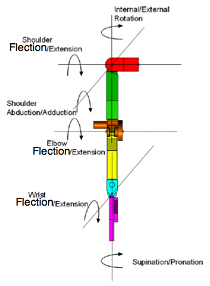
\includegraphics{figures/balta_arm_scheme} 
\caption[Scheme of Baltazar anthropomorphic arm]{Scheme of Baltazar anthropomorphic arm with available rotation \acp{DOF}.}
\label{img:balta_arm_scheme}
\end{figure}

\begin{figure}
\centering
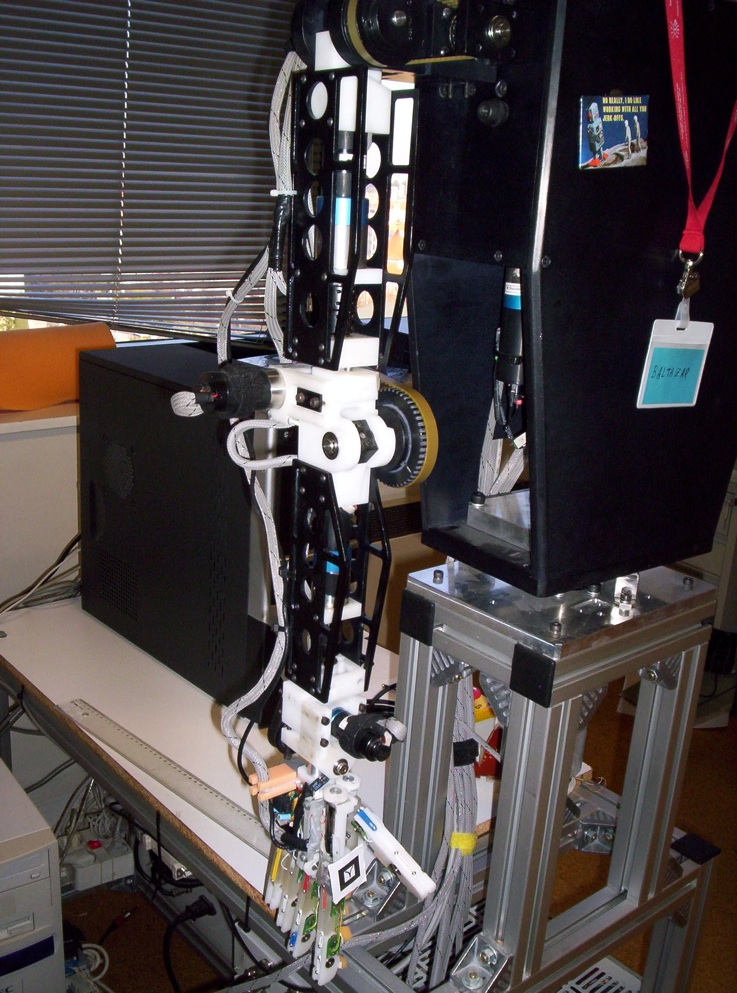
\includegraphics{figures/balta_arm_real} 
\caption[Real Baltazar anthropomorphic arm]{Real anthropomorphic arm of Baltazar.}
\label{img:balta_arm_real}
\end{figure}

Fig.~\ref{img:balta_real_cad} shows the robotic platform Baltazar in its entirety, whereas a scheme and a picture of the arm can be seen in Fig.~\ref{img:balta_arm_scheme} and in Fig.~\ref{img:balta_arm_real}, respectively.

\label{balta_ee}
The intersection between the two last motor axes, at the base of the wrist, is considered the end-effector for Baltazar.\index{Baltazar!end-effector}

Forward and inverse kinematics of the robotic arm are taken into account. This arm, which aims to replicate a human one, consists of 6 joints:
\begin{itemize}
\item 2 joints are associated with the shoulder;

\item 2 with the elbow; and

\item 2 with the wrist.
\end{itemize}

As far as this work is concerned, forward kinematics will be used as an extra tool or constraint to the iterative inverse kinematics solution which will be detailed later. The purpose is to exclude those solutions that do not respect a specific restriction imposed on the position of some joints. This is done to operate the robot easily and with no risk of damage when it is close to other objects, such as a table.

%%%%%%%%%%%%%%%%%%%%%%%%%%%%%
\subsection{Anthropomorphic Arm Forward Kinematics}
\index{Baltazar!anthropomorphic arm!forward kinematics}

\begin{table}
\caption[\acs{SDH} parameters of Baltazar anthropomorphic arm]{A possible \ac{SDH} parameterization of the anthropomorphic arm of Baltazar, derived during this thesis work in order to make use of existing robotics tools.}
\label{tab:balta_arm_sdh}
\centering
\medskip
\begin{tabular}{*{5}{l}} % table with 5 left-aligned columns
\toprule
Link $i$ & $a_i$ [cm] & $d_{i+1}$ [cm] & $\alpha_i$ [$\degree$] & $\theta_{i+1}$ [$\degree$] \\
\otoprule
$0$ & $0$ & $0$ & $\pi/2$ & $-\pi/2$ \\
\midrule
$1$ & $0$ & $0$ & $\pi/2$ & $\pi/2$ \\
\midrule
$2$ & $2.82$ & $29.13$ & $\pi/2$ & $\pi/2$ \\
\midrule
$3$ & $2.18$ & $0$ & $\pi/2$ & $\pi$ \\
\midrule
$4$ & $0$ & $26.95$ & $\pi/2$ & $\pi/2$ \\
\midrule
$5$ & $0$ & $0$ & $0$ & $-\pi/2$ \\
\bottomrule
\end{tabular}
\end{table}

A possible \ac{SDH} parameterization of Baltazar 6-\acs{DOF} arm, written down for this thesis work in a way similar to how the iCub arm kinematics was derived\footnote{\url{http://eris.liralab.it/wiki/ICubForwardKinematics}}, is shown in Table~\ref{tab:balta_arm_sdh}. Similarly, an \ac{MDH} parameterization for the anthropomorphic arm is shown in Table~\ref{tab:balta_arm_mdh}.

\begin{table}
\caption[\acs{MDH} parameters of Baltazar anthropomorphic arm]{A possible \ac{MDH} parameterization of the anthropomorphic arm of Baltazar, taken from~\cite{lopes:2004}.}
\label{tab:balta_arm_mdh}
\centering
\medskip
\begin{tabular}{*{5}{l}} % table with 5 left-aligned columns
\toprule
Joint $i$ & $a_{i-1}$ [cm] & $d_i$ [cm]& $\alpha_{i-1}$ [$\degree$] & $\theta_i$ [$\degree$] \\
\otoprule
$1$ & $0$ & $0$ & $0$ & $0$ \\
\midrule
$2$ & $0$ & $0$ & $\pi$ & $\pi/2$ \\
\midrule
$3$ & $0$ & $29.13$ & $\pi$ & $\pi/2$ \\
\midrule
$4$ & $2.82$ & $0$ & $\pi$ & $0$ \\
\midrule
$5$ & $-2.18$ & $26.95$ & $-\pi$ & $\pi/2$ \\
\midrule
$6$ & $0$ & $0$ & $\pi$ & $0$ \\
\bottomrule
\end{tabular}
\end{table}



%%%%%%%%%%%%%%%%%%%%%%%%%%%%%
\subsection{Anthropomorphic Arm Inverse Kinematics}
\index{Baltazar!anthropomorphic arm!inverse kinematics}
\label{sec:balta_arm_inv_kin}

The inverse kinematics problem is that of computing the joint angles\footnote{For a robot whose joints are all rotational, like the one used in this work.} that a robot configuration should present, given a spatial position and orientation of the end-effector. This is a useful tool for manipulator path planning, more so than forward kinematics.

One problem is that, in general, the inverse kinematic solution is non-unique, and for some manipulators no closed-form solution exists at all. If the manipulator possesses more \acp{DOF} than the number strictly necessary to execute a given task, it is called \emph{redundant} and the solution for joint angles is under-determined. On the other hand, if no solution can be determined for a particular manipulator pose, that configuration is said to be \emph{singular}. Typically, a singularity is due to an alignment of axes reducing the effective \acp{DOF}.

We address inverse kinematics in two steps. First, we set the anthropomorphic arm to the desired position (positioning of wrist); then, we change its orientation to a suitable one (orientation of hand).

Let $\mathbf{P}$ denote the desired position of the wrist, and $\mathbf{Z}$ be a null vector. In homogeneous coordinates, this means that:
%
\begin{gather}
\mathbf{P} = \begin{bmatrix} x & y & z & 1 \end{bmatrix}^T, \\
\mathbf{Z} = \begin{bmatrix} 0 & 0 & 0 & 1 \end{bmatrix}^T.
\end{gather}

The position of the wrist, $\mathbf{P}$, can be related to the various joint angles by cascading the different homogeneous coordinate transformation matrices:
%
\begin{equation}\label{eq:wrist_pos}
\mathbf{P} = \prod_{i=0}^5 \quad \leftidx{^i}{\mathbf{T}}_{i+1} \quad \mathbf{Z},
\end{equation}
%
where, as per Eq.~\ref{eq:transf}, $\leftidx{^i}{\mathbf{T}}_{i+1}$ denotes homogeneous transformation between frames $i+1$ and $i$.

In order to achieve a desired 3D location, the first four joints of the arm (counting from the shoulder) must be set to a specific position. Like~\cite{lopes:2004}, we will use the following transcendental result iteratively in order the determine these positions. Equation
%
\begin{equation}
a \cos(\theta) + b \sin(\theta) = c 
\end{equation}
%
has solutions
%
\begin{equation}\label{eq:transc}
\theta = 2 \arctan \left( \frac{b \pm \sqrt{a^2+b^2+c^2}}{a+c} \right).
\end{equation}

Eq.~\ref{eq:transc} is useful for determining the joint angles of an inverse kinematics problem. Notice that this equation has two solutions: the desired joint position can be chosen accordingly to the physical limits of a joint and/or by using additional criteria (comfort, least change).

To position the arm wrist to a given position $\mathbf{P}$ in space, we need to determine the corresponding values of joints $\theta_1, \theta_2, \theta_3, \theta_4$. Given the kinematic structure of the anthropomorphic arm of Baltazar, the distance $\rho$ from the base to the wrist (end-effector) depends only on $\theta_4$. Using Eq.~\ref{eq:wrist_pos}, the following constraint holds:
%
\begin{equation}\label{eq:theta4value}
a \cos(\theta_4)+  b \sin(\theta_4) = \rho^2 - (a_2^2 + l_2^2 + l_1^2 + a_1^2),
\end{equation}
%
where
\begin{equation}
\begin{eqsystem}
a = 2 (- a_2 a_1 + l_2 l_1) \\
b = - 2 (l_2 a_1 + a_2 l_1).
\end{eqsystem}
\end{equation}

Since Eq.~\ref{eq:theta4value} is compatible with the transcendental Eq.~\ref{eq:transc}, we can determine the value of $\theta_4$.

The solution of $\theta_2$ and a constraint on $\theta_3$ are obtained from the $z$ component (third column) of $\mathbf{P}$, obtained from Eq.~\ref{eq:wrist_pos}. In order for the parameters in Eq.~\ref{eq:transc} to permit the existence of a $\theta_2$ solution, we need $\theta_3$ to be such that:
%
\begin{gather}
a^2 + b^2 + c^2 > 0 \label{eq:theta3constraint} \\
\begin{eqsystem}
a = d_2 \cos(\theta_4) + l_2 \sin(\theta_4) - d_1 \sin(\theta_3) \\
b = - d_1 \sin(\theta_4) + l_2 \cos(\theta_4) + l_1\\
c = z.
\end{eqsystem}
\end{gather}

The algorithm that computes inverse kinematics consists in initializing $\theta_3$ in such a way that the constraint of Eq.~\ref{eq:theta3constraint} holds, subsequently allowing the computation of the remaining joint angles~\cite{carreiras:predgrab}.


All the computed angle variables are tested against the two solutions of Eq.~\ref{eq:transc}, so that we can verify if the values are coherent with the physical joint limits of the anthropomorphic arm (see Table~\ref{tab:balt_arm_joints} on p.~\pageref{tab:balt_arm_joints}).

As far as hand orientation is concerned, it is sufficient to constrain the solutions to a specific \emph{plane}, by specifying a normal vector to the plane as an input of the inverse kinematics software solver. Note that, in this way, one \ac{DOF} is still free (hand palm up or hand palm down).

%%%%%%%%%%%%%%%%%%%%%
%%%%%%%%%%%%%%%%%%%%%
\section{Hardware Devices of Baltazar}
\index{Baltazar!hardware devices}

\subsection{``Flea'' Cameras}

\begin{figure}
\centering
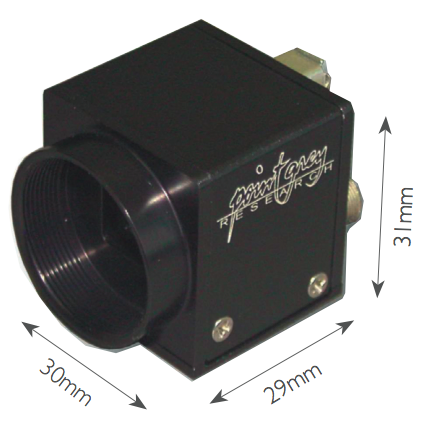
\includegraphics[scale=0.4]{figures/flea}
\caption[Point Grey ``Flea'' camera]{Point Grey ``Flea'' camera. The small dimensions of these cameras is worth noting, making it possible to employ them as (moving) humanoid eyes.}
\label{img:flea}
\end{figure}

Two colour cameras are attached on each of the eyes of Baltazar. These are ``Flea'' cameras, manufactured by Point Grey Research and displayed in Fig.~\ref{img:flea}. They are equipped with an IEEE-1394 FireWire interface and the following characteristics:
\begin{itemize}
\item very compact size: $30 \times 31 \times 29$ mm;

\item 1/3'' Sony \ac{CCD} sensor;

\item high processing speed, up to $640 \times 480$ resolution at 60 \ac{FPS};

\item external trigger, strobe output;

\item 12-bit \ac{ADC}.
\end{itemize}


\begin{figure}
\centering
\subfloat[][``Flea'' camera seen from above.]
{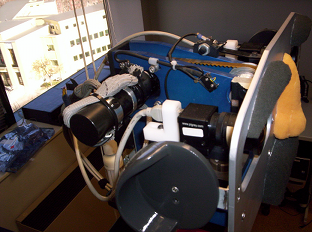
\includegraphics[width=.90\columnwidth]{figures/balta_cam_above} \label{img:balta_cam_above} } \\
%
\subfloat[][``Flea'' camera seen from below.]
{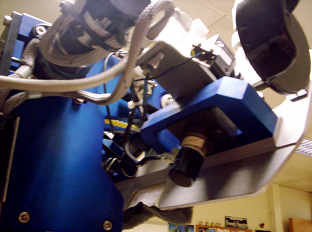
\includegraphics[width=.90\columnwidth]{figures/balta_cam_below} \label{img:balta_cam_below} }
%
\caption[Right eye Baltazar camera]{Right eye Baltazar camera as seen from two perspectives.}
\label{fig:balta_cam}
\end{figure}


%TODO: insert specification table and explain how we came to our custom params

%%%%%%%%%%%%%%%%%
\subsection{Controller Devices}

%NMCTest.exe => COM4 = hand; COM 1 = arm

\begin{figure}
\centering
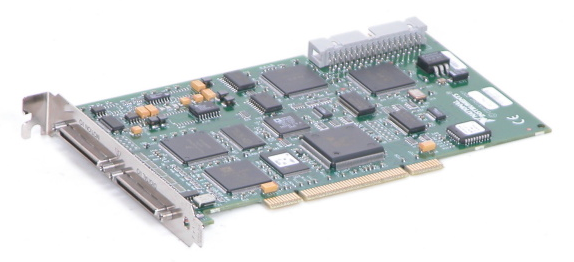
\includegraphics[scale=0.5]{figures/ni7340}
\caption[National Instruments 7340 Motion Controller]{National Instruments 7340 Stepper/Servo Motion Controller.}
\label{img:ni7340}
\end{figure}

The four \acp{DOF} of the head of Baltazar correspond to four axes or encoders; these are managed by a National Instruments PCI-7340 motion control board, shown in Fig.~\ref{img:ni7340}.

The 7340 controller is a combination servo and stepper motor controller for PXI, Compact PCI, and PCI bus computers. It includes programmable motion control for up to four independent or coordinated axes of motion, with dedicated motion I/O for limit and home switches and additional I/O for general-purpose functions. Servo axes can control:
\begin{itemize}
\item servo motors;

\item servo hydraulics;

\item servo valves and other servo devices.
\end{itemize}

Servo axes always operate in closed-loop mode. These axes use quadrature encoders or analog inputs for position and velocity feedback and provide analog command outputs with a standard range of $\pm 10$ V.

Stepper axes of the 7340 controller, on the other hand, can operate in open- or closed-loop mode. In closed-loop mode, they use quadrature encoders or analogue inputs for position and velocity feedback (in closed-loop only), and they provide step/direction or clockwise/counter-clockwise digital command outputs. All stepper axes support full, half, and microstepping applications.

The 7340 controller reflects a dual-processor architecture that uses a 32-bit CPU, combined with a \ac{DSP} and custom \acp{FPGA}, all in all providing good performance.

\bigskip

With regards to application software for this controller, the bundled tool NI-Motion is used. NI-Motion is a simple high-level programming interface (\acs{API}) to program the 7340 controller. Function sets are available for LabVIEW~\cite{link:labview} and other programs.

LabVIEW is a platform and development environment for a visual programming language (also from National Instruments) called ``G''. 

%\subsection{Limb control board}

In order to actuate the anthropomorphic arm and hand of Baltazar, another control board is mounted on the platform. The \ac{NMC} communication protocol\footnote{\url{http://www.jrkerr.com/overview.html}} is used to control the six joints of the limbs of the robot.

%\verb!TODO: add picture!

\begin{table}
\caption[Joint angles in Baltazar arm server]{Joint angles as available in Baltazar arm \acs{YARP} server. The ``physical limits'' are the actual angle limitations of the real robot joints, while the ``original bounds'' column indicates the limits that had been theoretically planned in Lopes \emph{et al.}~\cite{lopes:2004}, for the sake of historical reference.

All angles are expressed in degrees.}
\label{tab:balt_arm_joints}
\centering
\medskip
\begin{tabular}{*{5}{l}} % table with left-aligned columns
\toprule
encoder & description & arm joint & physical limits & original bounds \\
\otoprule
1 & shoulder abduction/adduction & 1 & [-45 35] & [-45 135] \\
\midrule
2 & shoulder extension/flection & 2 & [-40 5] & [-110 10] \\
\midrule
3 & not used & - & - & - \\
\midrule
4 & torso rotation & - & - & - \\
\midrule
5 & shoulder external/internal rotation & 3 & [-90 0] & [-90 0] \\
\midrule
6 & elbow extension/flection & 4 & [-90 0] & [-90 0] \\
\midrule
7 & arm pronation/supination & 5 & [-80 80] & [-90 90] \\
\midrule
8 & wrist extension/flection & 6 & [-29 45] & [-45 45] \\
\bottomrule
\end{tabular}
\end{table}

%%%%%%%%%%%%%
%%%%%%%%%%%%%
\section{Software Setup}

During the development of a piece of software, particularly if it is a project involving different people and institutions as well as operating systems and hardware, one should keep in mind certain basic principles of software engineering\index{software engineering} at all times:
\begin{itemize}
\item high cohesion;

\item low coupling

\item explicit interfacing;

\item information hiding.
\end{itemize}

Some software libraries that were largely employed in the development of this project (chiefly the \acs{YARP} set of libraries) will now be briefly presented.

%%%%%%%%%%
\subsection{YARP}
\label{sec:yarp} \index{YARP}

The iCub software (and other projects developed under the ``umbrella'' of the \ac{RobotCub} Consortium, such as this thesis) is potentially parallel and distributed. Apart from \acp{API} that speak directly to the hardware, the upper layers might require further support libraries, as is often necessary when programming robot systems immersed in various computer networks. In fact, many software solutions are already available~\cite[Table~1]{calisi:2008}. In the case of \ac{RobotCub}, these missing libraries include \emph{middleware}\index{middleware} mechanisms and were custom developed: their suite is called \ac{YARP}.

\ac{YARP} is open source\index{open source} and, as such, it is suitable for inclusion of newly developed iCub code. The rationale in this choice lays in the fact that having the source code available and, especially, well understood, can potentially simplify the software integration activity.

In order to facilitate the integration of code, clearly the simplest way would be to lay out a set of standards and to ask developers to strictly follow them. In a large research project like \ac{RobotCub}, the community should also allow for a certain freedom to developers, so that ideas can be tested quickly. These two requirements are somehow conflicting. Especially, they are conflicting when different behaviours are to be integrated into a single system and the integrator is not the first developer.

To allow developers to build upon the already developed behaviours, the researchers of \ac{RobotCub}\index{RobotCub} chose to layer the software and release-packaged behaviours in the form of \acp{API}. The idea is to produce behaviours that can be used without necessarily getting into the details of the middleware code employed. While for lower levels there is no much alternative than following a common middleware approach, higher levels and user level code can be developed by considering a less demanding scenario. In the latter case, modules are distributed with interfaces specified in an \ac{API}---possibly a C++ class hierarchy.

\begin{figure}
\centering
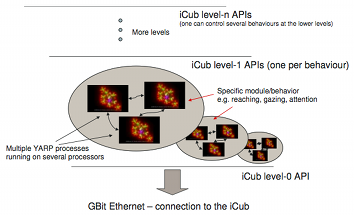
\includegraphics{figures/icub_sw_arch}
\caption[Software architecture of the iCub]{Software architecture of the iCub (and \acs{RobotCub}).}
\label{img:icub_sw_arch}
\end{figure}

Internally, each module will unleash a set of YARP processes and threads whose complexity will be hidden within the module. Various levels of configuration are possible. In one case, the given module would be capable of running on a single processor machine. This is a tricky and difficult choice since in many cases the behaviour of the robot relies explicitly on timing, synchronization, and performances of its submodules. Considering that eventually each module is a very specialized controller, issues of real-time performances have to be carefully evaluated. The modules' \acp{API} will include tests and indications on the computational timing and additional requirements in this respect, to facilitate proper configuration and use.

Fig.~\ref{img:icub_sw_arch} exemplifies the iCub software architecture. The lowest level of the software architecture consists of the level-0 \ac{API} which provides the basic control of the iCub hardware by formatting and unformatting IP packets into appropriate classes and data structures. IP packets are sent to the robot via a Gbit Ethernet connection. For software to be compliant to the iCub, the only requirement is to use this and only this \ac{API}. The \ac{API} is provided for both Linux and Windows. The iCub behaviours/modules/skills will be developed using \ac{YARP} to support parallel computation and efficient \ac{IPC}. \ac{YARP} is both open source\index{open source} and portable (i.e., OS independent), so it fits the requirements of \ac{RobotCub} in this sense. Each module can thus be composed of several processes running on several processors. 

\ac{YARP} is an open source framework for efficient robot control, supporting distributed computation and featuring a middleware infrastructure~\cite{link:yarp, metta:yarp}.

\ac{YARP} was created for a number of reasons:
\begin{itemize}
\item computer multitasking: it is useful to design a robot control system as a set of processes running on different computers, or several central processing units (CPUs) within a single system;

\item making communication between different processes easy;

\item code decoupling and modularity: it is a good practice to maintain and reuse small pieces of code and processes, each one performing a simple task. With \ac{YARP} it is easy to write location-independent modules, which can run on different machines without code changes whatsoever;

\item possibility to redistribute computational load among CPUs, as well as to recover from hardware failures.
\end{itemize}

In particular, as far as communication is concerned, \ac{YARP} follows the \emph{Observer} design pattern\index{observer design pattern|see{publish/subscribe}} (also known as \emph{publish/subscribe}\index{publish/subscribe}; see~\cite{gamma}). One or more objects (``observers'' or ``listeners'') are registered to observe an event that may be raised by the observed object (the ``subject'').

Several \emph{port} objects deliver messages to any number of observers, i.e., to their ports.

%%%%%%%%%%%%%%%%%%%%
\subsection{Other Software Libraries}

Besides \ac{YARP}, other libraries used for the implementation that are worth mentioning are \ac{GSL}\index{GSL}, its \ac{BLAS}\index{BLAS} interfaces, and OpenCV.

\bigskip

\ac{GSL} is a software library written in C for numerical calculations. Among other things, \ac{GSL} includes an implementation of the \ac{BLAS} interface.

\ac{BLAS}~\cite{link:blas} is a set of routines for linear algebra, useful to efficiently perform operations with vectors and matrices. They are divided into:
\begin{itemize}
\item Level 1 \ac{BLAS} for vector-vector operations;

\item Level 2 \ac{BLAS} for matrix-vector operations;

\item Level 3 \ac{BLAS} for matrix-matrix operations.
\end{itemize}

During the development of this thesis, \ac{GSL} and \ac{BLAS} were used to make computations between matrices fast and robust (preventing memory leaks and segmentation faults, thus improving security\index{security}).

OpenCV~\cite{link:opencv}\index{OpenCV} is a multi-purpose \ac{CV} library originally developed by Intel. Nowadays it is free for commercial and research use (under a BSD license). This library has two characteristics that it shares with \ac{RobotCub} research and that made us choose it:
\begin{itemize}
\item being cross-platform;

\item having a focus on real-time image processing. If OpenCV finds Intel's Integrated Performance Primitives (IPP) on the working system, it will use these commercial optimized routines to accelerate itself.
\end{itemize}